\documentclass[]{article}
\usepackage{lmodern}
\usepackage{amssymb,amsmath}
\usepackage{ifxetex,ifluatex}
\usepackage{fixltx2e} % provides \textsubscript
\ifnum 0\ifxetex 1\fi\ifluatex 1\fi=0 % if pdftex
  \usepackage[T1]{fontenc}
  \usepackage[utf8]{inputenc}
\else % if luatex or xelatex
  \ifxetex
    \usepackage{mathspec}
  \else
    \usepackage{fontspec}
  \fi
  \defaultfontfeatures{Ligatures=TeX,Scale=MatchLowercase}
\fi
% use upquote if available, for straight quotes in verbatim environments
\IfFileExists{upquote.sty}{\usepackage{upquote}}{}
% use microtype if available
\IfFileExists{microtype.sty}{%
\usepackage{microtype}
\UseMicrotypeSet[protrusion]{basicmath} % disable protrusion for tt fonts
}{}
\usepackage[margin=1in]{geometry}
\usepackage{hyperref}
\hypersetup{unicode=true,
            pdftitle={PREDICTING SALES VOLUMES},
            pdfauthor={Oriol Ordi and Alejandro Rojo},
            pdfborder={0 0 0},
            breaklinks=true}
\urlstyle{same}  % don't use monospace font for urls
\usepackage{graphicx,grffile}
\makeatletter
\def\maxwidth{\ifdim\Gin@nat@width>\linewidth\linewidth\else\Gin@nat@width\fi}
\def\maxheight{\ifdim\Gin@nat@height>\textheight\textheight\else\Gin@nat@height\fi}
\makeatother
% Scale images if necessary, so that they will not overflow the page
% margins by default, and it is still possible to overwrite the defaults
% using explicit options in \includegraphics[width, height, ...]{}
\setkeys{Gin}{width=\maxwidth,height=\maxheight,keepaspectratio}
\IfFileExists{parskip.sty}{%
\usepackage{parskip}
}{% else
\setlength{\parindent}{0pt}
\setlength{\parskip}{6pt plus 2pt minus 1pt}
}
\setlength{\emergencystretch}{3em}  % prevent overfull lines
\providecommand{\tightlist}{%
  \setlength{\itemsep}{0pt}\setlength{\parskip}{0pt}}
\setcounter{secnumdepth}{0}
% Redefines (sub)paragraphs to behave more like sections
\ifx\paragraph\undefined\else
\let\oldparagraph\paragraph
\renewcommand{\paragraph}[1]{\oldparagraph{#1}\mbox{}}
\fi
\ifx\subparagraph\undefined\else
\let\oldsubparagraph\subparagraph
\renewcommand{\subparagraph}[1]{\oldsubparagraph{#1}\mbox{}}
\fi

%%% Use protect on footnotes to avoid problems with footnotes in titles
\let\rmarkdownfootnote\footnote%
\def\footnote{\protect\rmarkdownfootnote}

%%% Change title format to be more compact
\usepackage{titling}

% Create subtitle command for use in maketitle
\providecommand{\subtitle}[1]{
  \posttitle{
    \begin{center}\large#1\end{center}
    }
}

\setlength{\droptitle}{-2em}

  \title{PREDICTING SALES VOLUMES}
    \pretitle{\vspace{\droptitle}\centering\huge}
  \posttitle{\par}
    \author{Oriol Ordi and Alejandro Rojo}
    \preauthor{\centering\large\emph}
  \postauthor{\par}
      \predate{\centering\large\emph}
  \postdate{\par}
    \date{2/12/2019}


\begin{document}
\maketitle

\hypertarget{introduction}{%
\section{Introduction}\label{introduction}}

This report will show the sales predictions in four different product
types and their relationship with service and costumer reviews. For this
purpose multipl regression will be used to build machine learning models
running three different algorithms (\emph{K-NN}, \emph{SVM} and
\emph{Random Forest}).

\hypertarget{objectives}{%
\paragraph{Objectives}\label{objectives}}

\begin{itemize}
\tightlist
\item
  Predict sales of four different product types: PC, Laptops, Netbooks
  and Smartphones.
\item
  Explain the services and customer reviews impact on sales of different
  product types.
\item
  Find and/or build the variables which better predicts sales volume.
\item
  Make recommendations to the sales department based in our results.
\end{itemize}

\hypertarget{materials}{%
\paragraph{Materials}\label{materials}}

For the development of this exercise the data sets provided by Danielle
Sherman via e-mail in .csv format will be used, consisting of the
following documents:

\begin{itemize}
\item
  \emph{existingprodutattributes2017.csv} -- This csv file contains
  information about product features, reviews and historical sales
  information. This file will be used to build the predictive models.
\item
  \emph{newproductattributtes2017.csv} -- This csv file contains
  information about product features and reviews, but no sales
  information. This is the data set where the model will be used to make
  the sales predictions.
\end{itemize}

\hypertarget{data-exploration}{%
\section{Data Exploration}\label{data-exploration}}

\hypertarget{missing-values}{%
\paragraph{Missing values}\label{missing-values}}

The existing products dataset has 15 observations that contain missing
values (NA). Since removing 15 observations in a 80 row dataset is
removing too much data, and considering that all missing values are in
the same attribute (\emph{BestSellersRank}), the best action is to
remove that attribute to deal with the missing values.

\hypertarget{outliers}{%
\paragraph{Outliers}\label{outliers}}

Most of the attributes have outliers, some of them a high number of
outliers. Removing all the outliers fro all the attributes would result
in reducing the dataset to almost no observations.\\
Therefore, only the outliers in the target variable (2 observations) are
removed.

\hypertarget{duplicates}{%
\paragraph{Duplicates}\label{duplicates}}

The dataset presents a few rows that are duplicated, except for the
price and (obviously) the product number. These rows are all
corresponding to the \emph{ProductType} ``Extended Warranty'' and they
are assumed to be different versions of the same product.\\
Thus, to avoid overfitting of the observations, the duplicated values
are all but one removed, and the remaining observation is used with the
\emph{Price} set to the mean of all prices in the duplicated
observations.

\hypertarget{missing-reviews}{%
\paragraph{Missing Reviews}\label{missing-reviews}}

There are 3 observations that have ``missing'' \emph{Star Reviews},
meaning that all the star attributes (\emph{x4StarReviews},
\emph{x3StarReviews}, \emph{x2StarReviews}, \emph{x1StarReviews}) are 0.

Since the nature of this missing data is not known, it is safer to
remove those observations from the dataset.

\hypertarget{abnormal-observations}{%
\paragraph{Abnormal Observations}\label{abnormal-observations}}

Plotting the \emph{Volume} against various indepenent variables shows
some interesting insights, namely that there are some observations that
don't align at all with the rest. One example of this can be seen in the
next figure, where the highest value of \emph{x1StarReviews} doesn't
align at all with the rest.

\begin{verbatim}
## `geom_smooth()` using method = 'loess' and formula 'y ~ x'
\end{verbatim}

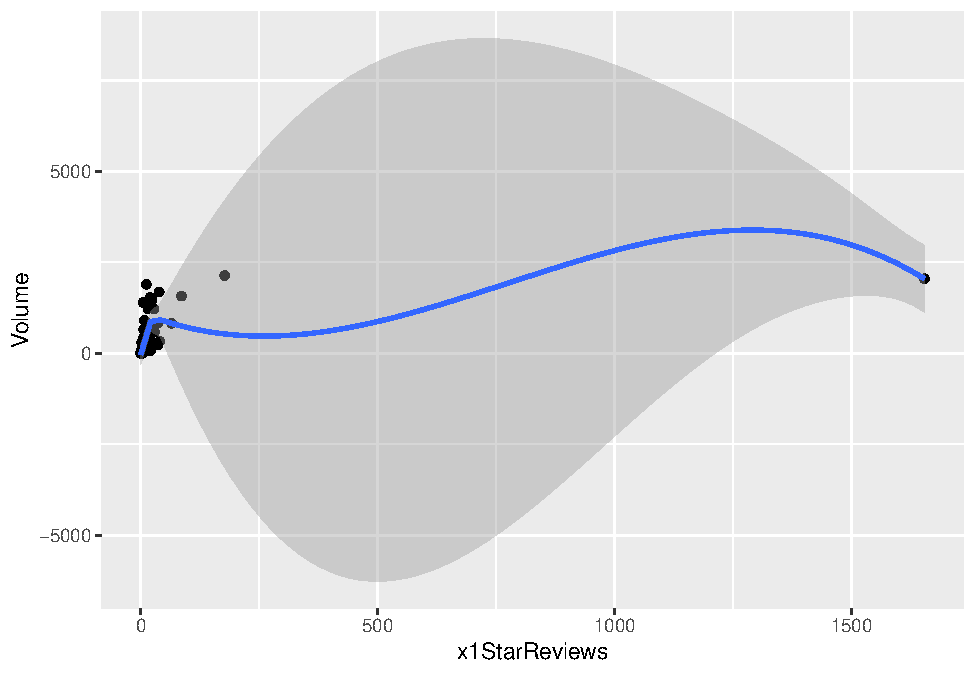
\includegraphics{final_predict_product_types_files/figure-latex/unnamed-chunk-2-1.pdf}

The observations that don't align for the model are, thus, removed from
the dataset.

\hypertarget{correlation}{%
\paragraph{Correlation}\label{correlation}}

To check correlation, including the \emph{ProductType}, the first thing
that has to be done is to dummify the \emph{ProductType}.\\
Once the \emph{ProductType} is dummified, the correlation between
variables can be checked:\\
\includegraphics{final_predict_product_types_files/figure-latex/unnamed-chunk-3-1.pdf}

In the correlation plot it can be seen that none of the \emph{Product
Types} are correlated with the \emph{Volume}. The next figure asserts
this affirmation:
\includegraphics{final_predict_product_types_files/figure-latex/unnamed-chunk-4-1.pdf}

In the last figure, the sales \emph{Volume} are shown by \emph{Product
Number}, grouped (colored) by \emph{Product Type} in descending order.
As it can be seen, the color distribution is spread out, meaning that
there is little relation between the \emph{Product Types} and the sales
\emph{Volume}.

Once the correlation between \emph{Volume} and \emph{Product Type} is
assumed to be nonexistent, the correlation between other attributes and
\emph{Volume} are checked, as well as the collinearity between
attributes, and the correlations higher than 0.85 are selected to take
into consideration:

\begin{verbatim}
##              id                   key     value
## 1        Volume         x5StarReviews 1.0000000
## 2 x4StarReviews         x3StarReviews 0.9348952
## 3 x4StarReviews         x2StarReviews 0.8975588
## 4 x3StarReviews         x2StarReviews 0.9706185
## 5 x4StarReviews         x1StarReviews 0.8723360
## 6 x3StarReviews         x1StarReviews 0.9362148
## 7 x2StarReviews         x1StarReviews 0.9391297
## 8        Volume PositiveServiceReview 0.9105237
## 9 x5StarReviews PositiveServiceReview 0.9105237
\end{verbatim}

After so much data preprocessing and eliminating observations, the
variables start to show high collinearity.

First of all, the \emph{x5StarReviews} has a correlation coefficient of
1 with the target variable, meaning that, most likely, the data was
tampered with and this attribute should not be trusted.

Then, as the correlation coefficients show, all the \emph{Star Review}
attributes are highly collinear.

Besides that, it is noteworthy that the \emph{PositiveServiceReview}
attribute has high correlation with the target variable and, thus, it is
possibly the best suited to explain the model.

The \emph{Star Review} variables have also semi-high correlation with
the target variable, but, since they are all collinear, only one of them
can be used. In this case, it will be the \emph{x4StarReviews}, which is
the most correlated with the \emph{Volume}.

\hypertarget{feature-engineering}{%
\paragraph{Feature engineering}\label{feature-engineering}}

New features have been built and tried with the goal of finding if there
are better predictors for sales volume. Various combinations of
different attributes (e.g.~\emph{Product Volume}, \emph{Density}, the
difference between \emph{Positive Service Reviews} and \emph{Negative
Service Reviews}, different forms of variable scaling, etc.).

\hypertarget{modelling}{%
\section{Modelling}\label{modelling}}

To find a model that best suits the data, several algorithms (namely
\emph{K-nn}, \emph{Random Forest} and \emph{SVM}) are used on various
combinations of variables.

For the sake of simplification, only a few relevant variables are
included in the following plot (although many more have been tried).

\includegraphics{final_predict_product_types_files/figure-latex/unnamed-chunk-7-1.pdf}

The best model is the one where Volume is explained by
\emph{x4StarReviews} and \emph{TotalServiceReviews}
(\emph{TotalServiceReviews} is the addition of
\emph{PositiveServiceReviews} and \emph{NegativeServiceReviews}) and the
algorithm used is \emph{Random Forest}. The RMSE in this case is 118,
the R-squared 0,96 and the MAE 74.

The following table shows the numerical results of the graph above:

\begin{verbatim}
##      metric                                                    model
## 1      RMSE                               Volume ~ x4StarReviews knn
## 2  Rsquared                               Volume ~ x4StarReviews knn
## 3       MAE                               Volume ~ x4StarReviews knn
## 4      RMSE                                Volume ~ x4StarReviews rf
## 5  Rsquared                                Volume ~ x4StarReviews rf
## 6       MAE                                Volume ~ x4StarReviews rf
## 7      RMSE                         Volume ~ x4StarReviews svmLinear
## 8  Rsquared                         Volume ~ x4StarReviews svmLinear
## 9       MAE                         Volume ~ x4StarReviews svmLinear
## 10     RMSE       Volume ~ x4StarReviews + PositiveServiceReview knn
## 11 Rsquared       Volume ~ x4StarReviews + PositiveServiceReview knn
## 12      MAE       Volume ~ x4StarReviews + PositiveServiceReview knn
## 13     RMSE        Volume ~ x4StarReviews + PositiveServiceReview rf
## 14 Rsquared        Volume ~ x4StarReviews + PositiveServiceReview rf
## 15      MAE        Volume ~ x4StarReviews + PositiveServiceReview rf
## 16     RMSE Volume ~ x4StarReviews + PositiveServiceReview svmLinear
## 17 Rsquared Volume ~ x4StarReviews + PositiveServiceReview svmLinear
## 18      MAE Volume ~ x4StarReviews + PositiveServiceReview svmLinear
## 19     RMSE         Volume ~ x4StarReviews + TotalServiceReviews knn
## 20 Rsquared         Volume ~ x4StarReviews + TotalServiceReviews knn
## 21      MAE         Volume ~ x4StarReviews + TotalServiceReviews knn
## 22     RMSE          Volume ~ x4StarReviews + TotalServiceReviews rf
## 23 Rsquared          Volume ~ x4StarReviews + TotalServiceReviews rf
## 24      MAE          Volume ~ x4StarReviews + TotalServiceReviews rf
## 25     RMSE   Volume ~ x4StarReviews + TotalServiceReviews svmLinear
## 26 Rsquared   Volume ~ x4StarReviews + TotalServiceReviews svmLinear
## 27      MAE   Volume ~ x4StarReviews + TotalServiceReviews svmLinear
## 28     RMSE                       Volume ~ PositiveServiceReview knn
## 29 Rsquared                       Volume ~ PositiveServiceReview knn
## 30      MAE                       Volume ~ PositiveServiceReview knn
## 31     RMSE                        Volume ~ PositiveServiceReview rf
## 32 Rsquared                        Volume ~ PositiveServiceReview rf
## 33      MAE                        Volume ~ PositiveServiceReview rf
## 34     RMSE                 Volume ~ PositiveServiceReview svmLinear
## 35 Rsquared                 Volume ~ PositiveServiceReview svmLinear
## 36      MAE                 Volume ~ PositiveServiceReview svmLinear
##          value
## 1  308.6878854
## 2    0.7275657
## 3  207.9627106
## 4  232.8134776
## 5    0.8255693
## 6  158.0854728
## 7  267.9907140
## 8    0.7841048
## 9  142.1433361
## 10 140.8847457
## 11   0.9550922
## 12  86.9714286
## 13 168.1760388
## 14   0.9071959
## 15  98.2133092
## 16 118.3831172
## 17   0.9678883
## 18  87.1450621
## 19 136.5958212
## 20   0.9570008
## 21  94.0285714
## 22 115.1185890
## 23   0.9638300
## 24  71.2316222
## 25 178.6947234
## 26   0.8956365
## 27 112.5191093
## 28 119.6164519
## 29   0.9611747
## 30  84.2226455
## 31 155.9522975
## 32   0.9230128
## 33  92.4343708
## 34 115.9532173
## 35   0.9594773
## 36  80.5010107
\end{verbatim}

\hypertarget{discussion}{%
\paragraph{Discussion}\label{discussion}}

The Dataset presents very few observations. For practical purposes, a
model that works well within the limitation of the Dataset has been
found. However, due to the nature of the Dataset, a slight change in the
way that the model is built presents enormous differences in its
outcome.

Thus, this model should be used with care, taking into account that the
model would work much better with a much larger Dataset.

\hypertarget{results}{%
\section{Results}\label{results}}

Once the model is defined, the predictions for the new products can be
easily calculated.

Using the predictions, a calculation can be easily done to know the
predicted sales volume for the 4 product types of interest, as can be
seen in the following figure:

\includegraphics{final_predict_product_types_files/figure-latex/unnamed-chunk-10-1.pdf}

In the following chart the impact of customer and service reviews on
sales volume can be seen. It is observed that when \emph{Positive
Service Reviews} and \emph{4 Star Reviews} grow, the sales volume is
higher.

\includegraphics{final_predict_product_types_files/figure-latex/unnamed-chunk-11-1.pdf}

\hypertarget{conclusions}{%
\section{Conclusions}\label{conclusions}}

\begin{itemize}
\tightlist
\item
  The sales volume predictions for the new products have been found
  using a \emph{Random Forest} algorithm with the \emph{x4StarReviews}
  and the \emph{TotalServiceReviews}.
\item
  The customers and service review variables are strongly related with
  sales volume.
\item
  The recommendation to the sales department is to be wary with the
  predictions. The dataset has a lot of issues (small sample, outliers,
  duplicated values, etc.) that affect the model, the results and the
  predictions. It is advised to gather more data to get more realistic
  results for this analysis.
\end{itemize}


\end{document}
